\documentclass{article}
\usepackage{pgfplots}
\usepackage{amsmath,amssymb,amsfonts}
\pgfplotsset{compat=1.17}

\begin{document}

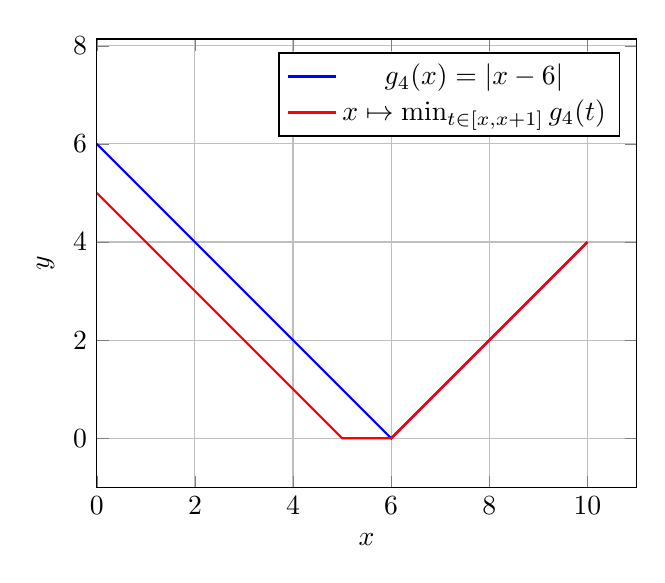
\begin{tikzpicture}
  \begin{axis}[
      axis equal,
      xlabel=$x$,
      ylabel=$y$,
      % title=Function Plots,
      grid=major,
      legend pos=north east,
      xmin=0,
      ymin=-1,
    ]
    
    \addplot[blue, thick, domain=0:10, samples=1001, sharp plot] {abs(x-6)};
    \addlegendentry{$g_{4}(x) = |x-6|$}

    \addplot[red, thick, domain=0:10, samples=1001, sharp plot] {%
      ifthenelse(x<5, 5-x,
        ifthenelse(x>6, x-6, 0)
      )
    };
    \addlegendentry{$x\mapsto\min_{t\in[x,x+1]} g_{4}(t)$}
    
  \end{axis}
\end{tikzpicture}

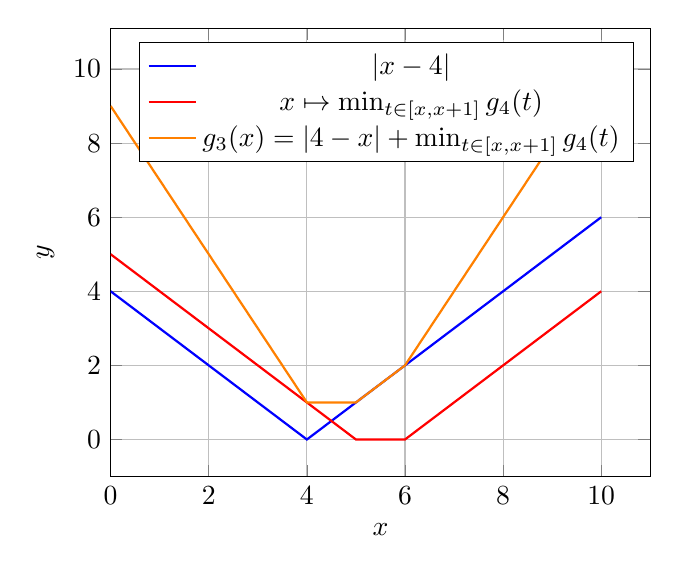
\begin{tikzpicture}
  \begin{axis}[
      % axis equal,
      xlabel=$x$,
      ylabel=$y$,
      % title=Function Plots,
      grid=major,
      legend pos=north east,
      xmin=0,
      ymin=-1,
    ]
    
    \addplot[blue, thick, domain=0:10, samples=1001, sharp plot] {abs(x-4)};
    \addlegendentry{$|x-4|$}

    \addplot[red, thick, domain=0:10, samples=1001, sharp plot] {%
      ifthenelse(x<5, 5-x,
        ifthenelse(x>6, x-6, 0)
      )
    };
    \addlegendentry{$x\mapsto\min_{t\in[x,x+1]} g_{4}(t)$}

    \addplot[orange, thick, domain=0:10, samples=1001, sharp plot] {abs(x-4) + (x<5 ? 5-x : (x>6 ? x-6 : 0))};
    \addlegendentry{$g_3(x) = |4-x| + \min_{t \in [x,x+1]} g_4(t)$}
  \end{axis}
\end{tikzpicture}

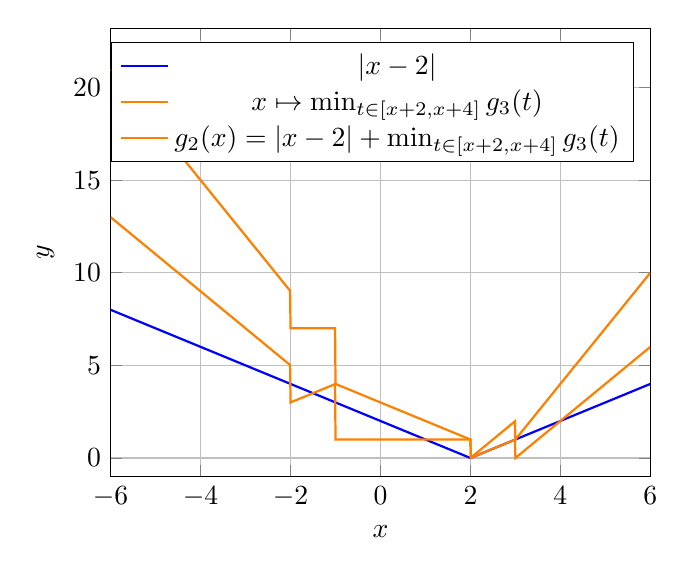
\begin{tikzpicture}
  \begin{axis}[
      % axis equal,
      xlabel=$x$,
      ylabel=$y$,
      % title=Function Plots,
      grid=major,
      legend pos=north east,
      xmin=-6,
      xmax=6,
      ymin=-1,
    ]

    \addplot[blue, thick, domain=-6:6, samples=1001, sharp plot] {abs(x-2)};
    \addlegendentry{$|x-2|$}

    \addplot[orange, thick, domain=-6:6, samples=1201, sharp plot]{(x<-2)*(1-2*x)
      + (x>=-2 && x<-1)*(x+5)
      + (x>=-1 && x<=2)*1
      + (x>2 && x<3)*(x-2)
      + (x>=3)*(2*x-6) };
    \addlegendentry{$x\mapsto\min_{t\in[x+2,x+4]} g_3(t)$}

    \addplot[orange, thick, domain=-6:6, samples=1201, sharp plot]{abs(x-2)+(x<-2)*(1-2*x)
+ (x>=-2 && x<-1)*(x+5)
+ (x>=-1 && x<=2)*1
+ (x>2 && x<3)*(x-2)
+ (x>=3)*(2*x-6)};
    \addlegendentry{$g_2(x) = |x-2| + \min_{t\in[x+2,x+4]} g_3(t)$}
  \end{axis}
\end{tikzpicture}


% \begin{tikzpicture}
%   \begin{axis}[
%       % axis equal,
%       xlabel=$x$,
%       ylabel=$y$,
%       % title=Function Plots,
%       grid=major,
%       legend pos=north east,
%       xmin=-6,
%       xmax=6,
%       ymin=-1,
%       xtick distance=1,
%       ytick distance=1,
%     ]

%     \addplot[blue, thick, domain=-6:6, samples=1001, sharp plot] {abs(x-1)};
%     \addlegendentry{$|x-1|$}

%     \addplot[orange, thick, domain=-6:6, samples=1001, sharp plot] { abs(x+2-2) + (x+2<-2)*(1-2*(x+2))
%       + (x+2>=-2 && x+2<-1)*(x+2+5)
%       + (x+2>=-1 && x+2<=0)*1
%       + (x+2>0 && x+2<3)*(x+2-2)
%       + (x+2>=3)*(2*(x+2)-6) };
%     \addlegendentry{$x\mapsto\min_{t\in[x+2,x+2]} g_2(t)$}

%     \addplot[green, thick, domain=-6:6, samples=1001, sharp plot] { abs(x-1)
%       + (x<-3)*(-2*x-5)
%       + (x>=-3 && x<-2)*(-x-2)
%       + (x>=-2 && x<=0)*0
%       + (x>0)*(2*x) };
%     \addlegendentry{$g_1(x) = |x-1| + \min_{t\in[x+2,x+2]} g_2(t)$}
%   \end{axis}
% \end{tikzpicture}

\end{document}